% !TEX root = ../../thesis.tex
\cleartoleftpage
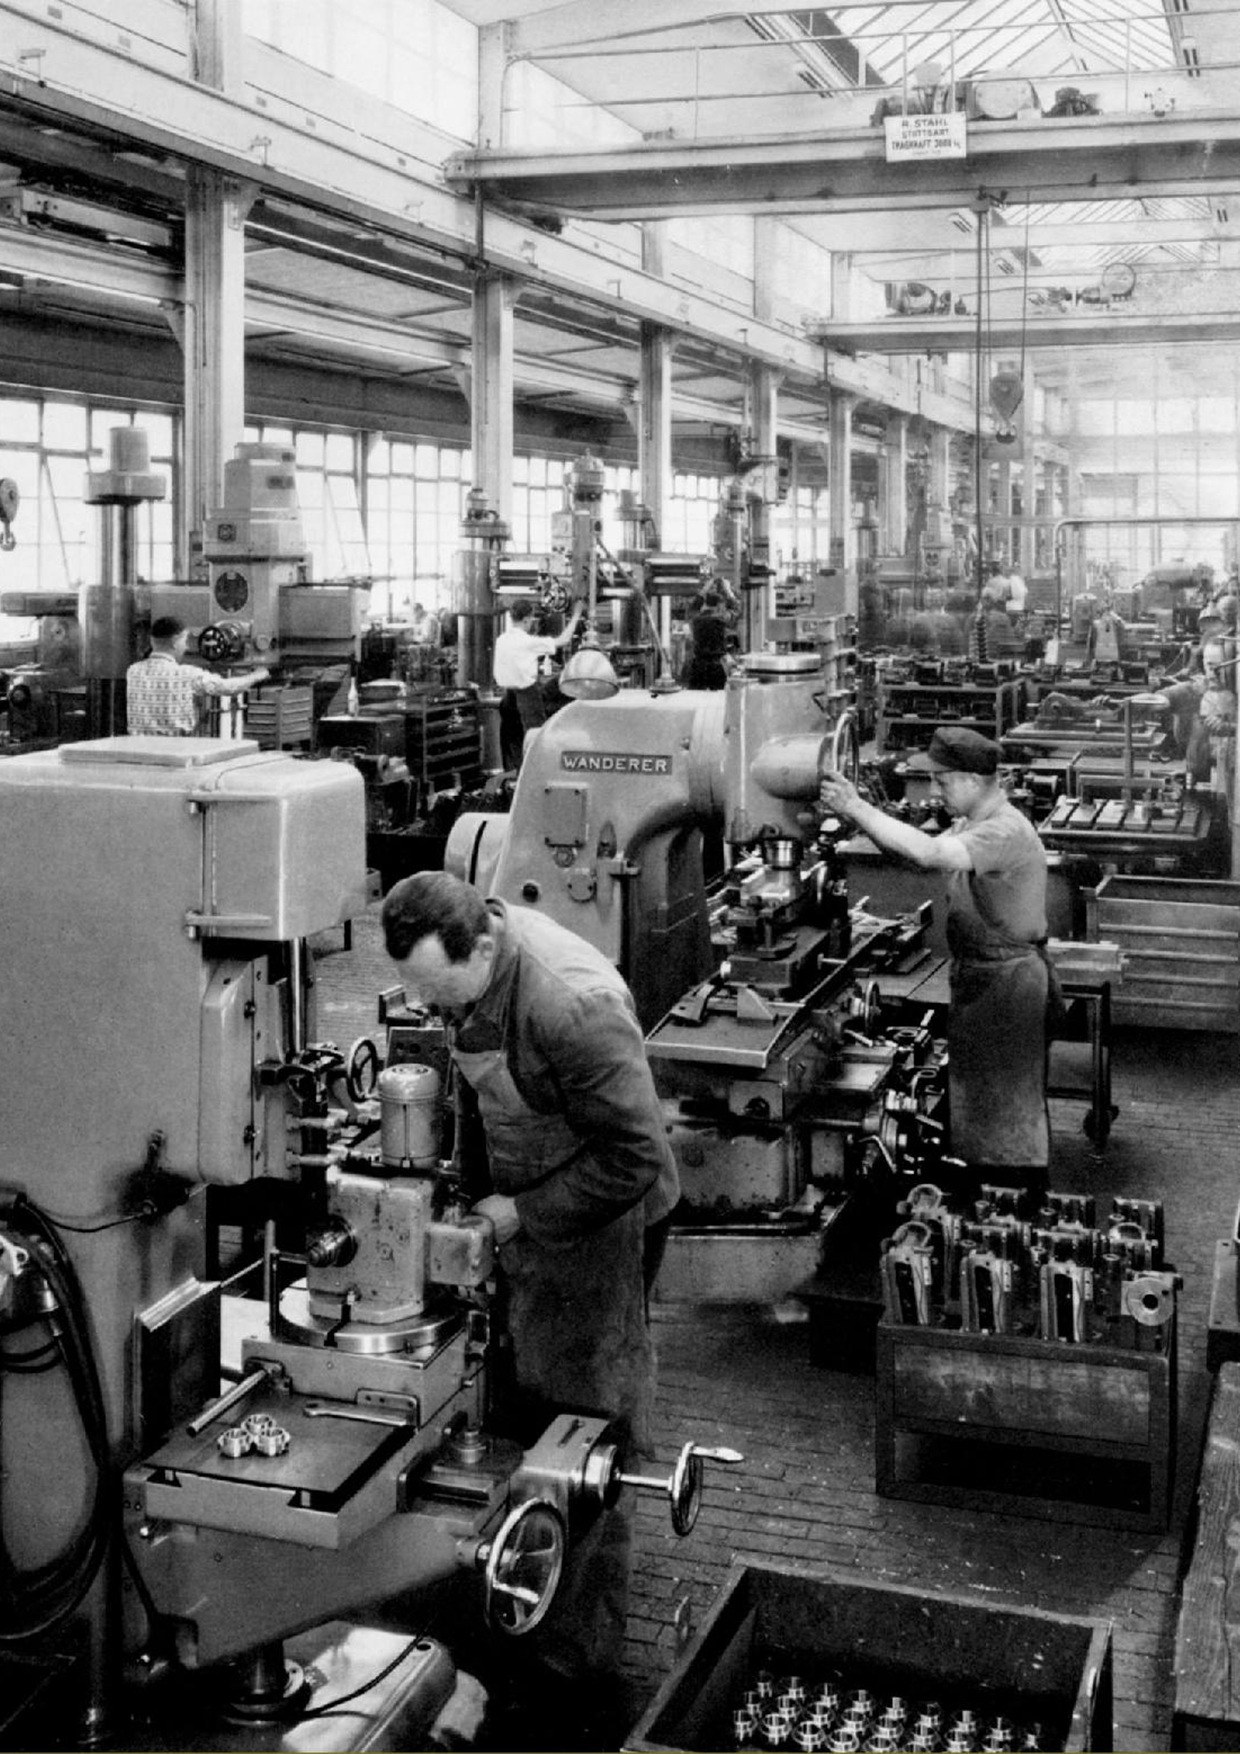
\includepdf{../media/chapter_illustration/old_factory}

\chapter{Motivations and Methodology}
\label{cha:methodology}

\section{Introduction} % (fold)

In chapter~\ref{cha:morphology-review}, we discussed the emergence of a novel paradigm in the field of robotics that appeared in the late eighties.  Embodied artificial intelligence rejects the symbolic approach and postulates that it is not possible to have intelligence without an actual robot body associated with its ecological niche~\parencite{pfeifer2001understanding}. Following this paradigm, several researchers have tried to tackle challenges in which the classical cognitivist approach failed (see \parencite{brooks1986achieving}) e.g. the understanding of natural forms of intelligence that require direct interaction with the real world.

Thus, an interesting evolution over recent decades is the demonstration of the importance of the morphology for sensorimotor control, cognition and development (\cite{kaplan2008corps}, \cite{steels1995artificial}, \cite{Pfeifer06}), which can be defined as follows:
\begin{formal}
    The morphology of a robot thus refers to the physical structure and form of a robot. Specifically, the focus is on characteristics such as link sizes, number of links, joint characteristics, mass distribution, actuator characteristics, material properties, sensor characteristics and sensor placements. In short, any characteristic that defines the physical structure of the robot is included in the term morphology.
    \signed{Chandana Paul~\parencite{paul2006morphological}}
\end{formal}

Exploring the interaction between body properties and cognition could lead both to a better understanding of animals’ behaviour (human beings in particular) and to build robots that are more adapted and robust to an open environment with unpredictable interactions. In particular, we can highlight the acquisition of sensorimotor tasks and the exploration of adapted bodies for natural, physical and social interactions with humans.

In this context, we should not only pay attention to the robot body design but \textbf{introduce morphology as an experimental variable and conduct experiments in the real world}. As Rodney Brooks said \emph{the world is its own best model}~\parencite{brooks1991intelligence} and simulators cannot handle the complexity of real physics with multi-point contacts, soft materials and frictions. This is especially true for complex dynamic tasks such as physical interaction or legged locomotion.

Following the definition of robotic morphology given by C. Paul, we need to find a framework allowing easy and quick tuning of morphological parameters on an actual robot in order to explore and hopefully find new ways of improving robot behaviour in the real world. However considering morphology as an experimental variable raised two major problems:
\begin{itemize}
    \item \textbf{how can we obtain an experimental robotic platform with both a morphology that can be changed easily and quickly and the capacity to act robustly in the real world? }
    \item \textbf{how can we make sure this platform, particularly the hardware, can be diffused and reused in the research community?}
\end{itemize}

In the next sections of this chapter, we will \textbf{suggest novel approaches and design processes to create and produce robotic platforms, the control and morphology of which can be freely explored through experimentation in the real world,  that are easy to  diffuse and reproduce in the research community.}
We will detail the methodological and design challenges involved in creating robots with variable and modular hardware. Then we will present the design methods we chose to address these challenges and those we have used to create Poppy (see chapter~\ref{cha:poppy-dev}). And finally, we will discuss the importance of open source distribution for creating open and cumulative science.


\section{Challenges} % (fold)

The role of morphology appears to be a fascinating open field of research but until now it has been under-explored.
We presented in chapter~\ref{cha:experimental-methods}, a review of robotic platforms, both commercial and lab prototypes. It appears the current platforms are not suitable to tackle these challenges.

Firstly, for most the electronic and mechanical structures are produced using classic manufacturing techniques,  which makes them too complicated and expensive to modify. Indeed, the classical way of designing and producing robots is a complicated, time-consuming and expensive process. The development of current robotic platforms requires dozens of engineers working for many years and significant fund-raising for production. Such techniques make creating variant parts impossible, mainly because of the approach and technologies chosen to design and produce them.


Secondly, beyond the restriction on exploring morphological variants, one of the fundamental aspects of the scientific research is to demonstrate facts, which should therefore be reproducible. Unfortunately in the robotics field, the amount of material resources and the techniques involved makes it difficult to transfer robot platforms from one lab to another. While commercial robots can be easily accessible (subject to appropriate funding) because they are relatively mass-produced, lab prototypes are mainly handcrafted and specifically tuned, which makes their  reproduction in another lab impossible. Therefore, scientific validation is limited and researchers cannot build novel work upon the one of their peers.

Finally, robot hardware of both types is very rarely open source, which simply prohibits any modification and reuse of the work (we will discuss more in detail the importance of this point in section~\ref{sec:allow-cumulative-science}).

Therefore, allowing  experimental platforms to be transferred and shared is a way of ensuring the scientific validity of experiments, and also of promoting and accelerating scientific research by reducing time lost in development, instead concentrating research resources on the exploration of novel ideas.


In this context, creating a platform reproducible everywhere without special tooling or skills, the morphology of which can be freely explored, raises methodological and design process challenges that we will describe in the following points.

\subsection{Make the morphology variable} % (fold)

Current robotic platforms, in particular humanoid ones, have mechanical parts either handcrafted or produced with classic machining techniques based on milling or casting metal alloys or plastic.
These techniques require specific upfront tooling which make the production of a small batch really expensive. Also, to keep the cost of the robot rather low, mass production is needed to achieve economy of scale. In this context, the morphology of current robotic platforms cannot be modified because it would require redoing most of the production process. In addition, the design of such mechanical parts is limited because the manufacturing process implies constraints and the complexity of a part greatly increases its cost. The same issues appear with electronics and the robot sensor space which is, in most cases, frozen. Thus the classic way to design and produce robot is not adapted to the free exploration of the robot morphology, novel design and production paradigm have to be used.


\subsection{Create reproducible robot prototypes} % (fold)

Most labs must reinvent the wheel by developing whole new robotic platforms even though functional setups have already been developeded by other laboratories and should/could be reused.

For example, several interesting robotic platforms explore key aspects of robot morphology. We can cite Kenshiro~\parencite{nakanishi2013design} which has a complex and bio-inspired artificial muscles actuator network, or semi-passive walkers such as Denise~\parencite{wisse2005three}, demonstrating impressive walking ability with little control and power actuation. Unfortunately, none of these robots can be and have ever been transferred to another lab. Indeed even if they were open source theirs productions require specific tooling and hand tuning that only few skilled people have.

Therefore some constraints have to be applied on hardware platforms to make them reproducible:
\begin{description}
    \item[Precision, stationary] Experiments should be repeatable, implying that the robot’s morphological properties should be stationary. This means that robot performance should not be dependent on where it was built or the users’ skills.
    \item[Easy and fast to duplicate:] In order for the platform to be reusable, it needs to be easy and fast to duplicate and not rely on specific tooling or exotic components.
    \item[Affordable:] To ensure widespread use, a key aspect is to keep the cost of the platform relatively low. The more labs involved, the better the scientific impact.
\end{description}


\subsection{Keep robotic platform simple and easy-to-use} % (fold)

The field of robotics is intrinsically multidisciplinary. A robot itself requires technology from mechanics, electronics and computer science, but the scientific impact of robotics can be far larger and reach non-engineering fields such as humanities, social or biological sciences. Thus, robotics is a specialised field  in which nobody can be an expert in all required skills.
We have to take into account the fact that the end user can certainly be expert in one specific subfield but a beginner in others. This mean that for each subfield, the designed robot has to be simple enough to be understood and used by beginners while having, at the same time, enough potential to not constrain users in their domain of expertise.



\section{The chosen design methods} % (fold)

To address these challenges, we suggest exploring an alternative design methodology that is driven by the desire to:
\begin{itemize}
    \item freely explore morphological properties,
    \item reduce the amount of time required between an idea and its experimentation on an actual robotic platform in the real world,
    \item make our work easily reproducible in any other lab,
    \item keep our work modular and free to use in accordance with open source principles, so it can be reused and extended for other projects.
\end{itemize}

To reach these goals, we decided to follow some design methods for both design and production, for all technological aspects of the robot (i.e. mechanics, actuation, electronics, software, distribution).

\subsection{3D-printed mechanical parts} % (fold)
We could envisage simply having classical mechanical parts that are reconfigurable and adjustable, allowing for example, the exploration of different lengths of a link or different centre of mass positions. However, this limits the morphological exploration to only a few dimensions with a limited range.

As we discussed in chapter REF, over the last few years, novel techniques, especially 3D printing have been revolutionizing the way we can produce objects. 3D printers not only open new horizons for the production of mechanical part, they are able to produce parts that were either not possible or extremely expensive with classical techniques (see \figurename~\ref{fig:complex_3D_printed_part}).It completely changes the paradigm associated with production. Indeed the cost does not change with the quantity or the complexity, meaning designers are free to explore the shape they want with almost no constraints.

\begin{figure}[tb]
\centering
    \subfloat[][Example of object those shape would be impossible to produce without additive manufacturing]{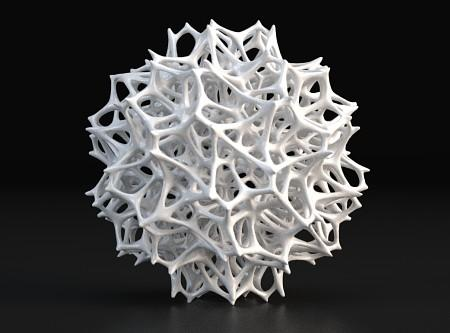
\includegraphics[width=0.4\linewidth]{complex_3Dprinted_part.jpeg}}
    \hfil
    \subfloat[][3D printed metal heat exchanger]{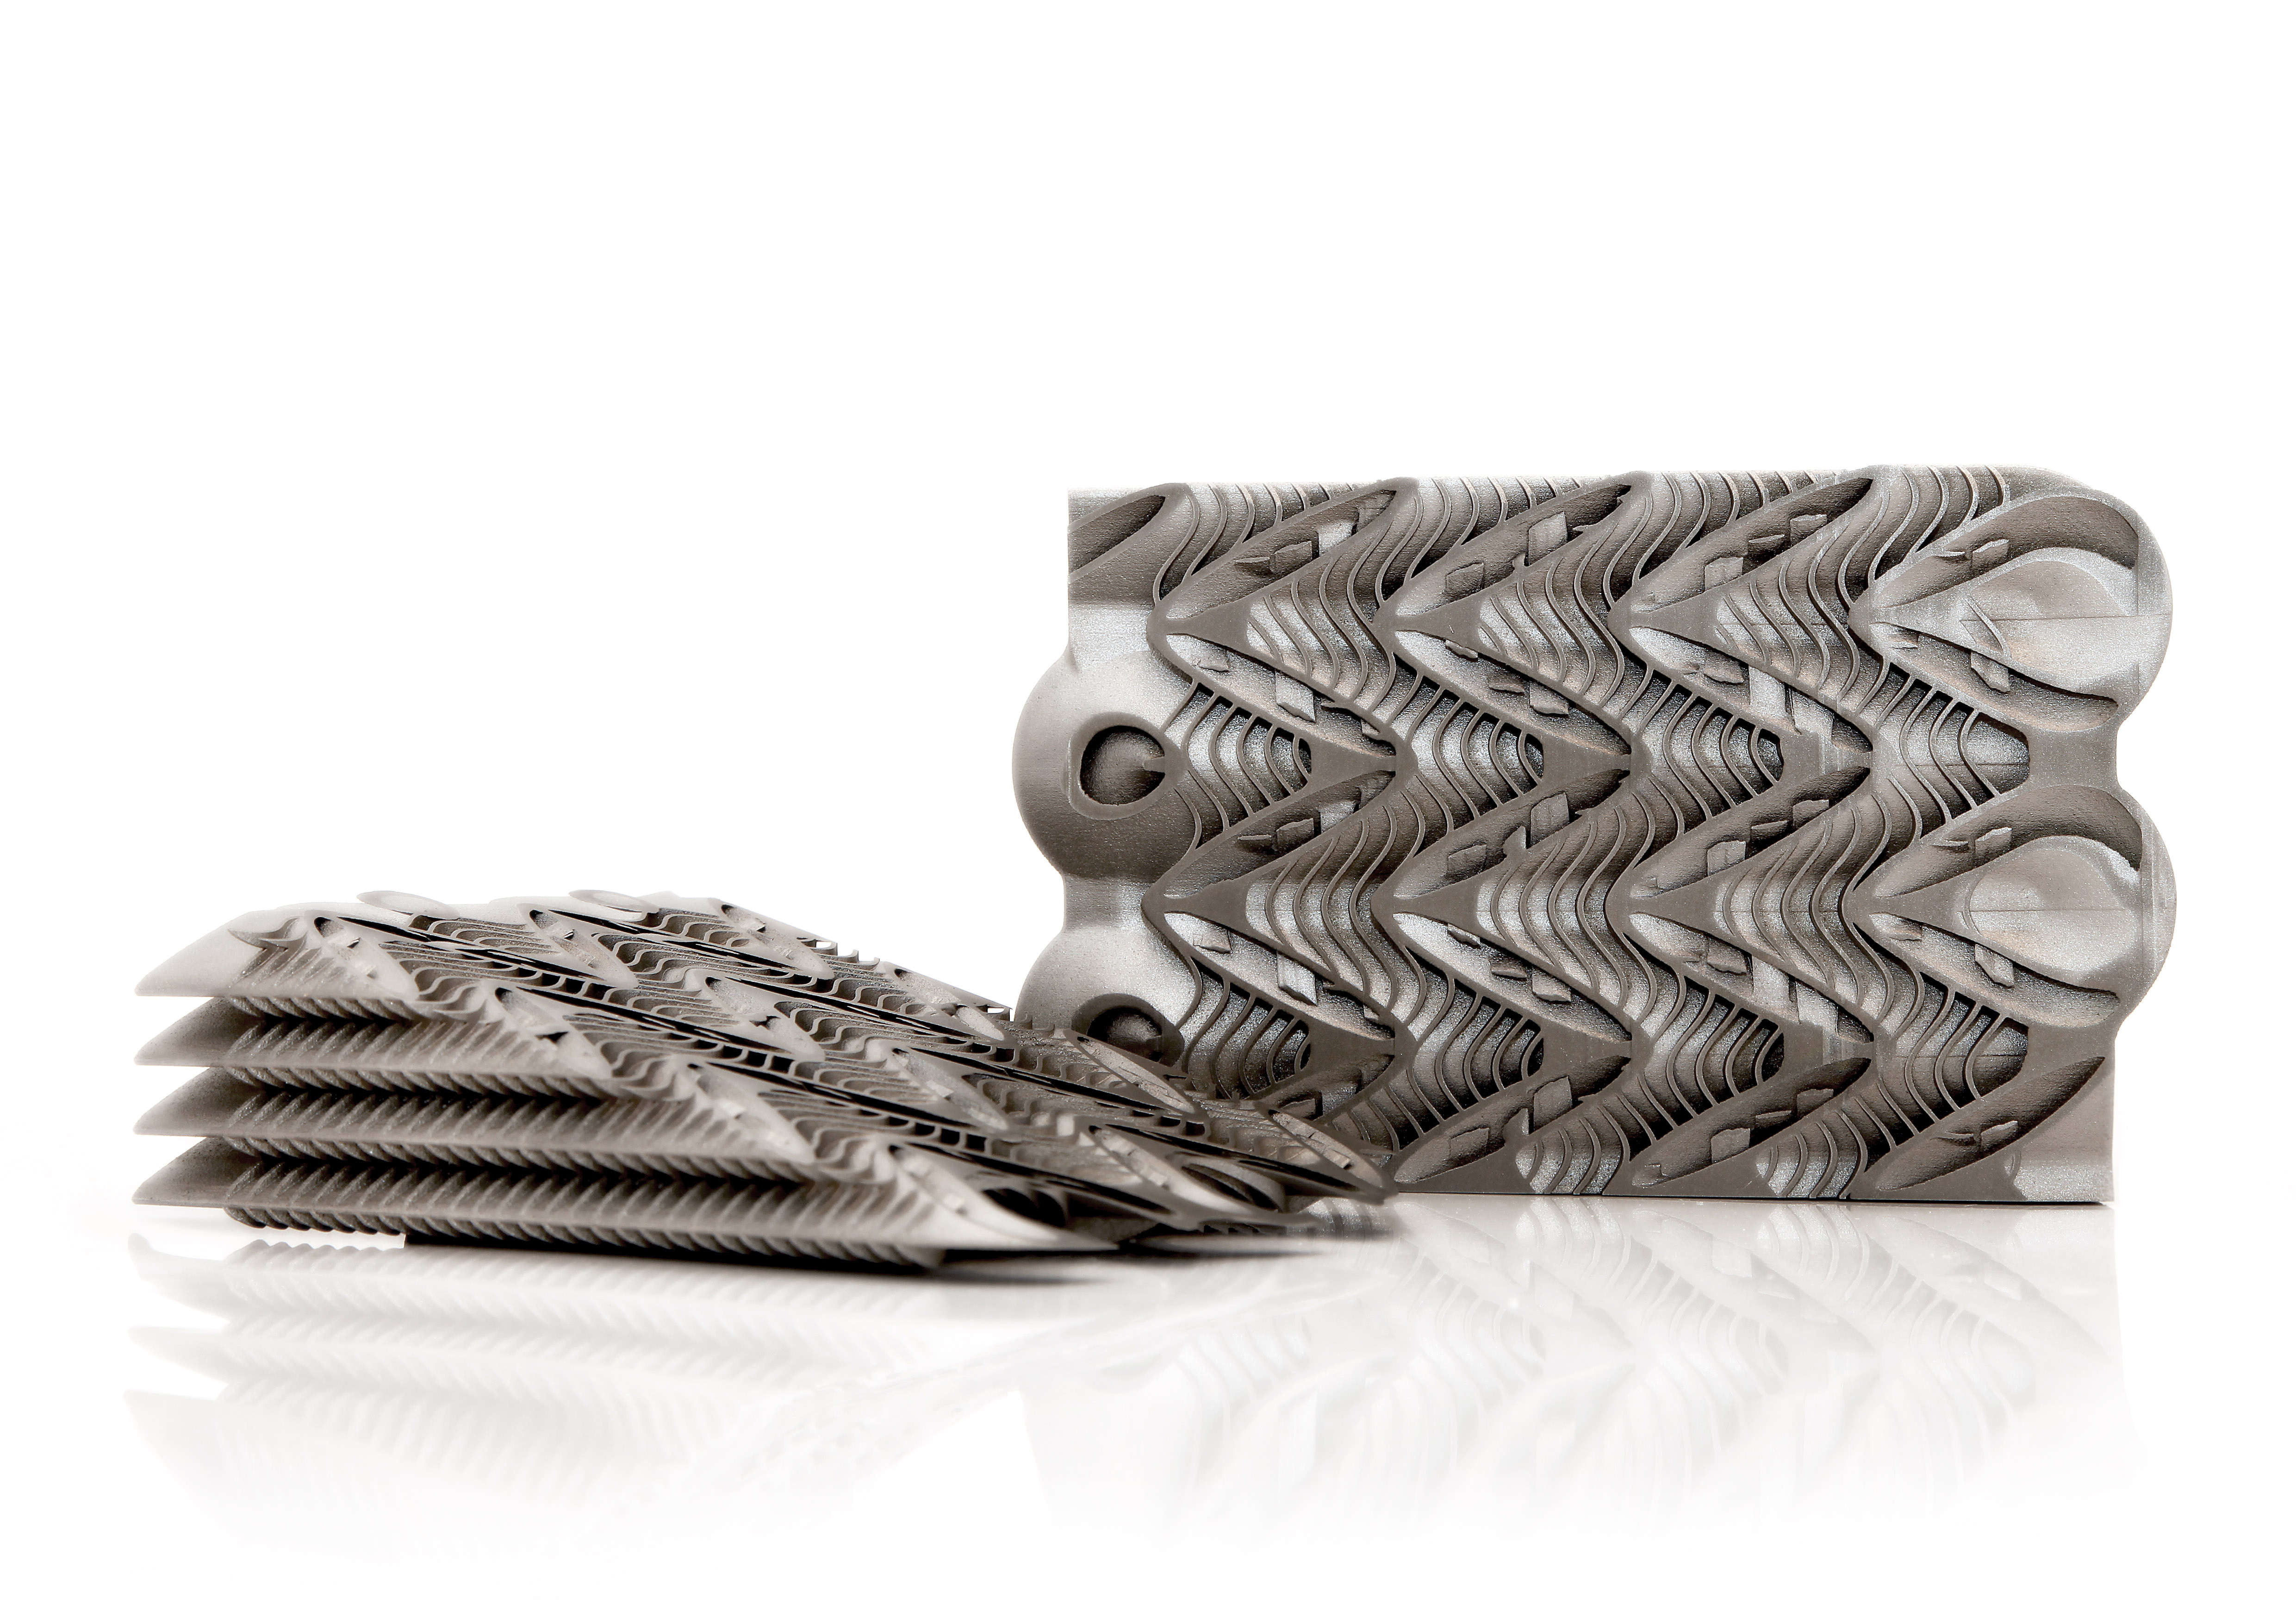
\includegraphics[width=0.55\linewidth]{complex_heat_exchanger.jpg}}
    \caption{Example of complex parts those production has been made possible by 3D printing techniques.}
    \label{fig:complex_3D_printed_part}
\end{figure}


Also, these novel techniques come with the open hardware and makers revolution, which has brought low cost 3D printers into the home. The production of mechanical parts can be now done in few hours directly on site with limited human handling (see \figurename~\ref{fig:conception_loop}).

\begin{figure}[tb]
    \begin{center}
        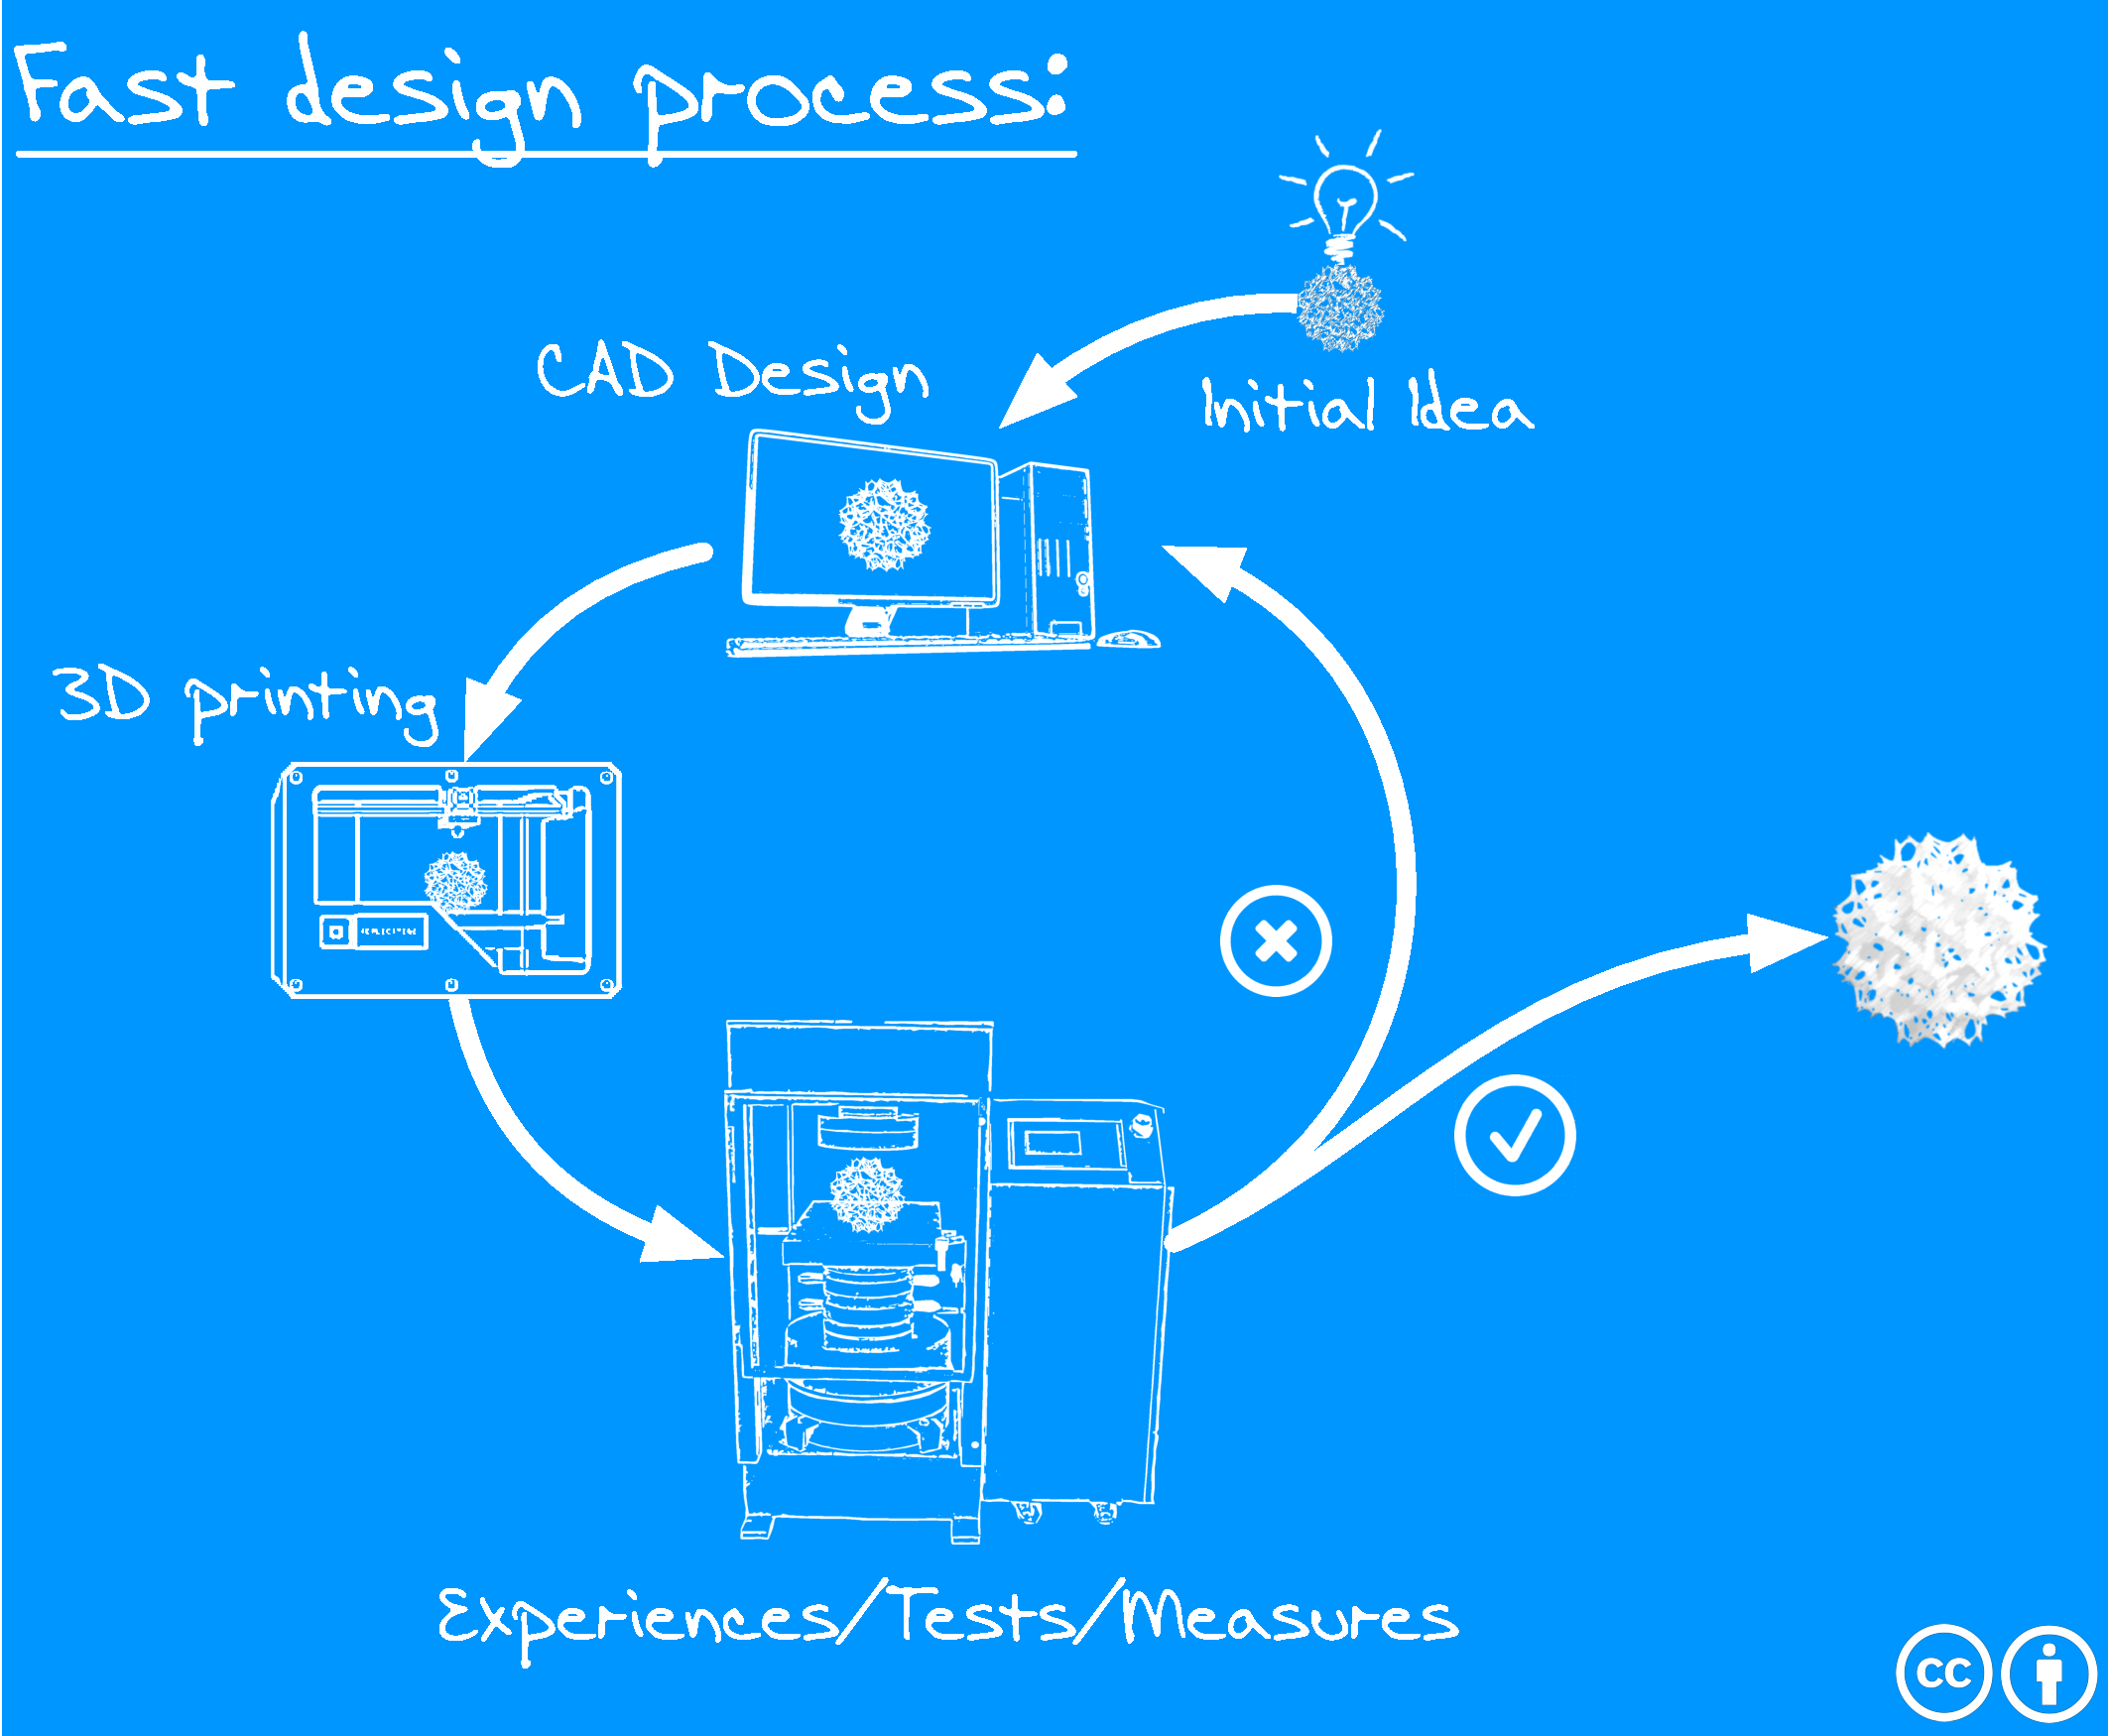
\includegraphics[width=\linewidth]{conception_iterative.pdf}
    \end{center}
    \caption{The 3D printing technique allows for fast iterative conception loop while it permits to directly and automaticcaly produce a prototype on site for a fraction of the cost of classical manufacturing techniques.}
    \label{fig:conception_loop}
\end{figure}

3D printers have several key abilities:
\begin{description}
    \item[Worldwide:] 3D printed parts can be obtained everywhere, either by personal printing or by ordering parts on other web services, such as i.materialise, shapeways or sclupteo.
    \item[Low cost:] The cost of producing 3D parts is rather low, ranging from tens of cents if produced on a personal printer to tens of euros if ordered though a web service.
    \item[Fast:] In a couple of hours a whole part can be created from scratch. When using web services, queuing and shipping delays have to be added, increasing the production time to several days.
    \item[Skill-free:] Since the production process is fully digital, few or no specialist skills are required.
    \item[Multi-material, precise and robust:] current 3D printers can create precise (up to 0.1mm) parts in different material such as nylon, PLA, ABS or even titanium and flexible material. The parts obtained are robust and can be used as final parts for several years.
    \item[Reduce the number of part:] 3D printing  can be used to print complex parts and even assembled parts as complex as bearings or gearboxes. This means we can replace multiple parts that have to be assembled into ready-to-use ones.
\end{description}

These properties of the 3D printing process allow for the first time to really explore morphological variants of mechanical parts. Indeed, it is now fast and low-cost to create alternative designs. Associated with modular architecture, we can easily and quickly change robot parts and conduct experiments. Also this process is compatible with our diffusion goals since it is simple, and accessible anywhere with an internet connection and a mailing address. Also parts can be produced directly in the lab if it is equiped with a 3D printer.


\subsection{Electronic architecture based on Arduino} % (fold)

Thanks to 3D printing, exploring morphological variants of mechanical parts is now easier than ever before but unfortunately, the printing of electronic components and boards is not yet available. However, exploring the role of morphology does not only concern the mechanical properties but also the sensors apparatus i.e. \textbf{which sensor is used and where is it placed on the body}. The Swiss bot (see REF) is a great example of the impact of the sensors’ positioning on robot behaviour.

To permit the exploration of sensor-system variants, we suggest basing the electronic architecture on Arduino. As presented in section~\ref{sec:arduino-review}, Arduino is an open-source electronics platform based on easy-to-use hardware and software. It is intended for anyone doing interactive projects. The Arduino board can sense the environment by receiving inputs from a wide variety of sensors, and affects its surroundings by controlling lights, motors, and other actuators. Low-level embedded programing skills are not required, since Arduino boards can be programmed using the Arduino programming language\footnote{\url{http://arduino.cc/en/Main/Software}} which abstracts all the complexity.

\begin{figure}[tb]
    \begin{center}
        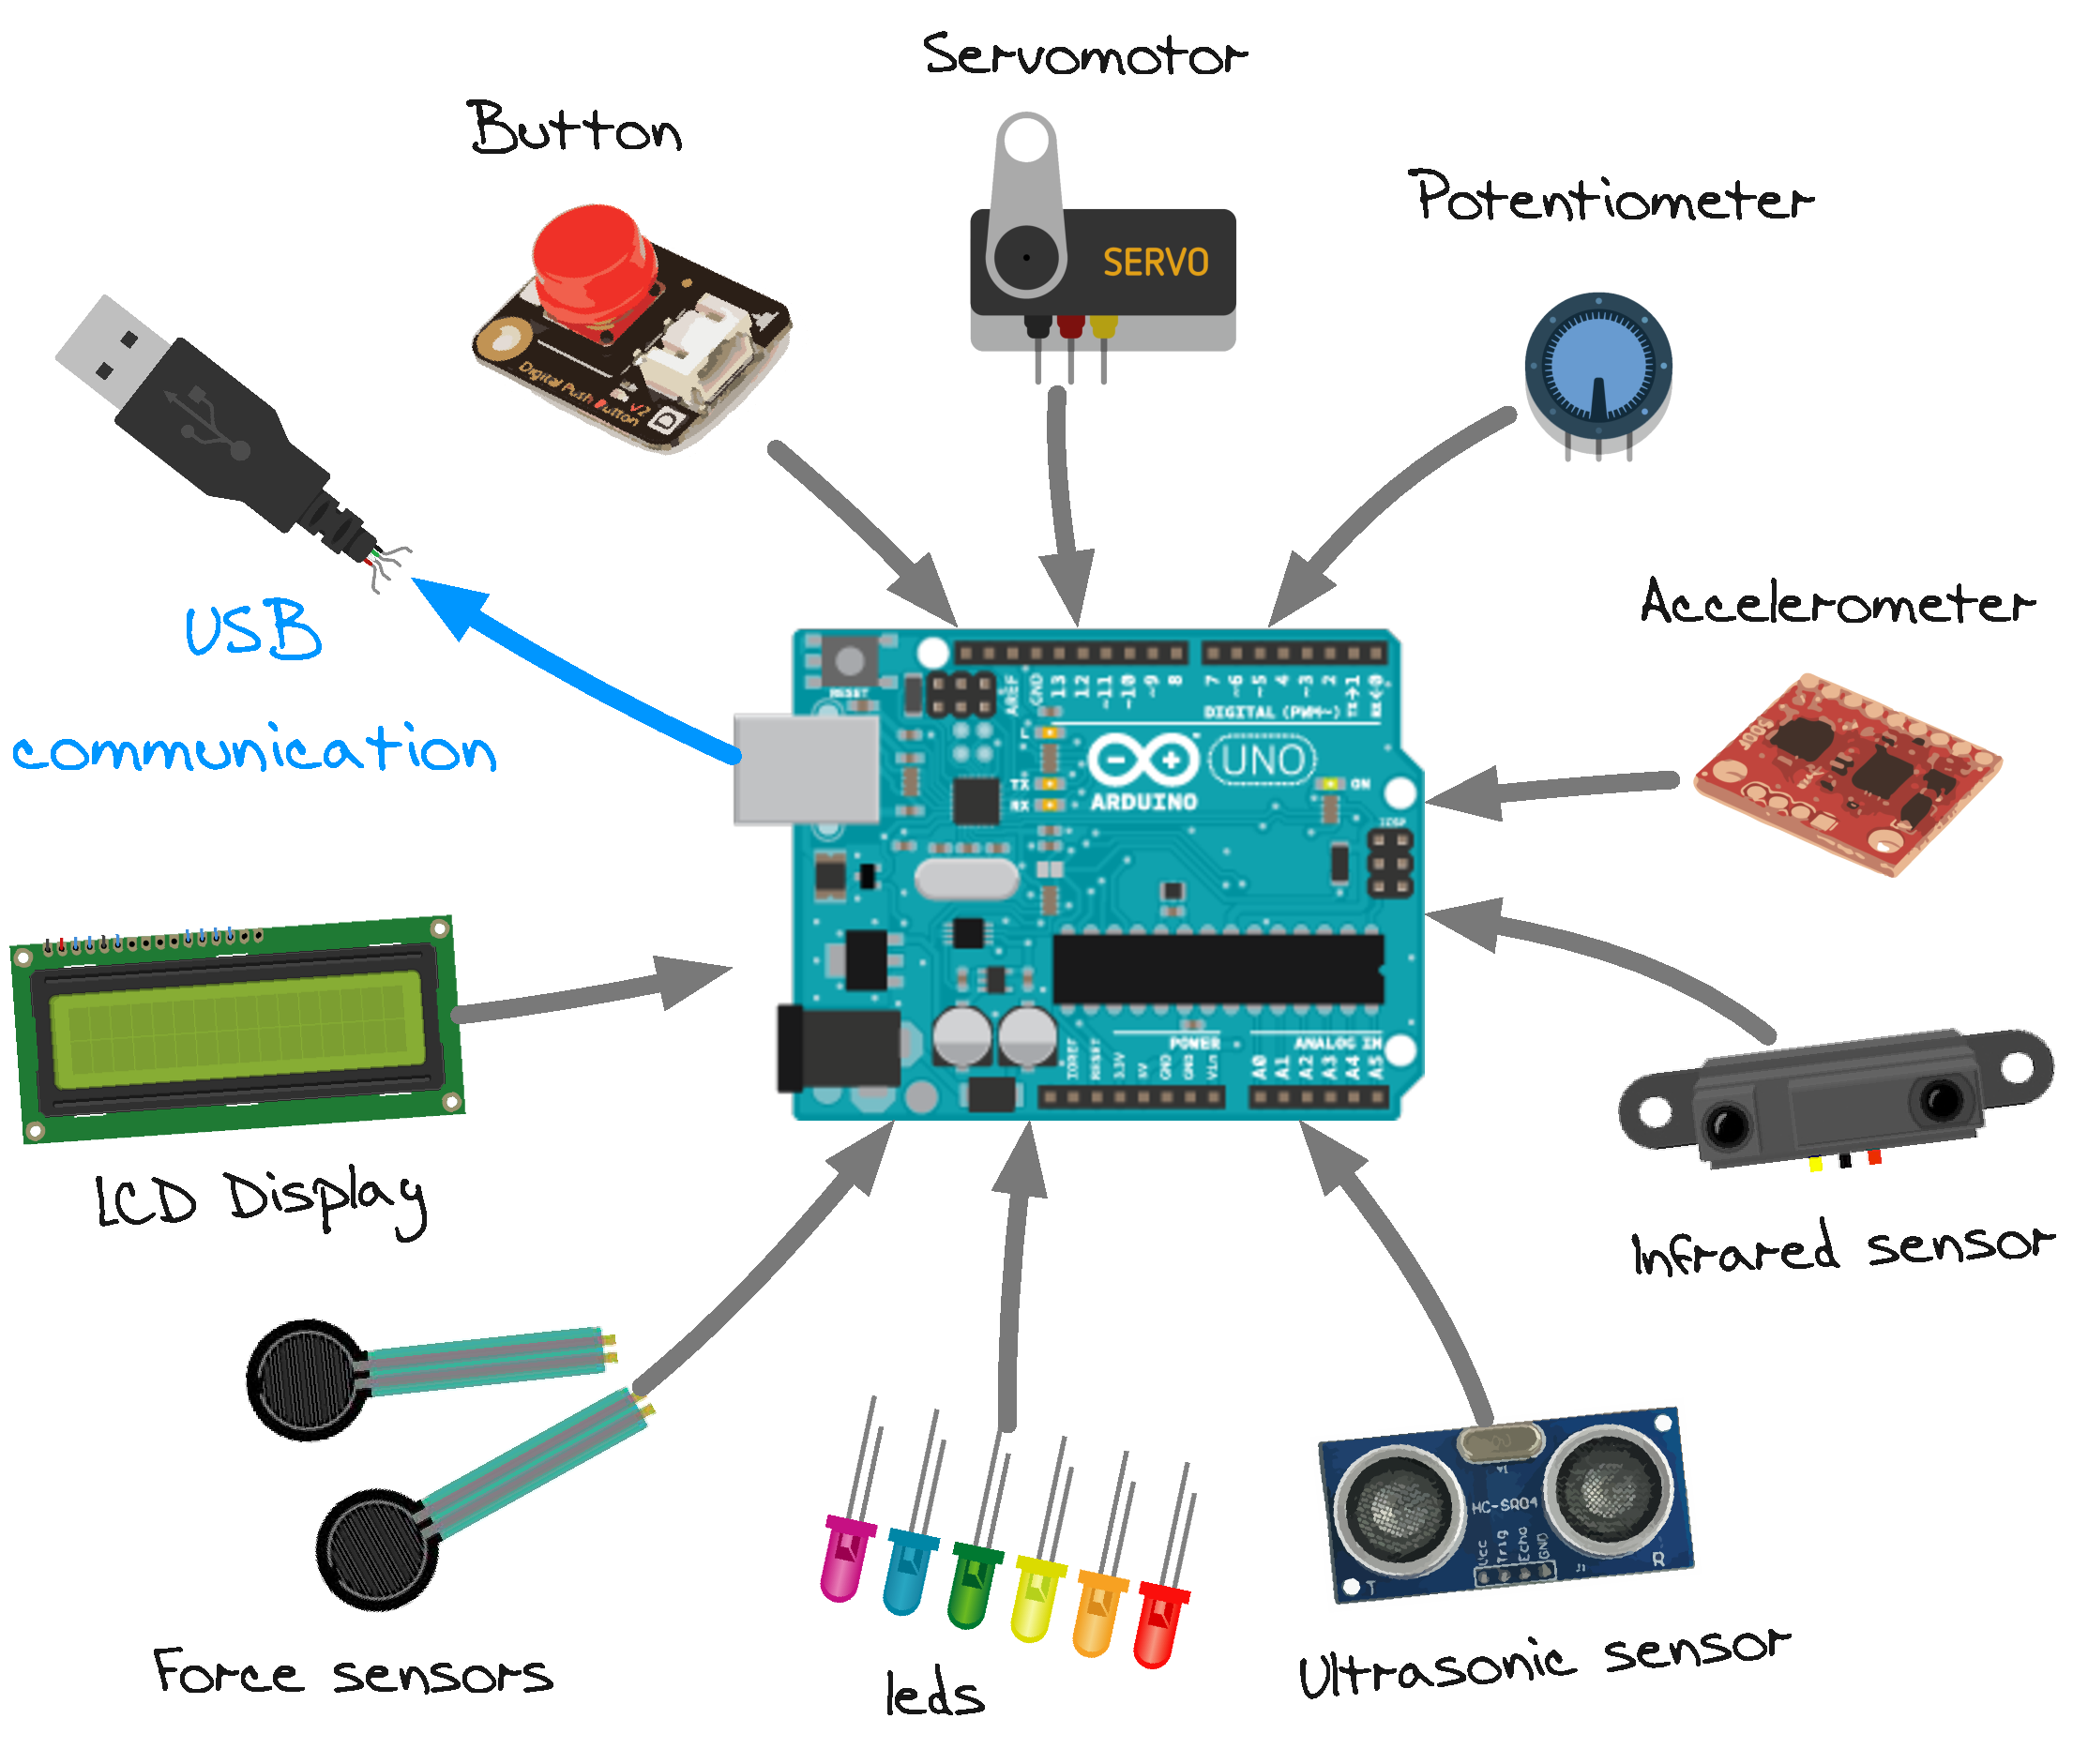
\includegraphics[width=0.9\linewidth]{arduino_electronique.pdf}
    \end{center}
    \caption{The use of Arduino as electronic architecture  allows for sensors to be easily added and/or changed, while keeping the same electronic board. In addition, it permits to add expressive components such as LEDs, LCD or sound systems, allowing users to easily explore human-robot interaction.}
    \label{fig:arduino_modular_electronic}
\end{figure}


The Arduino community is very active and expanding, more and more sensors are designed to be directly plugged onto Arduino boards. Thus, using Arduino adds modularity to robot electronic architecture, allowing the reconfiguration of the sensors space by easily adding new ones (see \figurename~\ref{fig:arduino_modular_electronic}).


\subsection{All-in-one actuators} % (fold)

% As we discussed in chapter~\ref{cha:experimental-methods},
Robots are actuated using various techniques from classic and cheap servomotors to the highly powerful and dynamic hydraulic actuators powering the Atlas humanoid robot.
While some actuator technologies such as Series Elastic Actuator (SEA), cable-driven or artificial muscles are really promising to create more robust and efficient robots, they are still work-in-progress solutions and require advanced skills both to assemble and use. These technologies are not yet compatible with the creation of diffusible and reproducible robotic platforms in a multidisciplinary research community.

% \textbf{TODO: Image de system mecanique avec cable ou air }

To permit the diffusion, we need off-the-shelf and stationary solutions, easy to assemble, easy-to-use and available anywhere. Also, to allow the exploration of morphology, actuators have to be modular and allow the tuning of several parameters.

We therefore chose to use Robotis Dynamixel servo-motors\footnote{\url{http://www.robotis.com/xe/dynamixel_en}} for robot actuation (see \figurename~\ref{fig:dynamixel_models}). Dynamixel motors are easily accessible, as they are mass produced and shipped worldwide. Also they are commonly used actuators in the robotic field and many robots are powered by them, including Darwin-OP~\parencite{ha2011development}, Myon~\parencite{hild2012myon} , Acroban~\parencite{ly2011bio} or Nimbro~\parencite{schwarznimbro}.

The Dynamixel motors are not simple servomotors, they are all-in-one-modules that contain drivers, encoders and communication buses. They are also quite powerful, robust and rather precise. This is achieved by the combination of Maxon motors, metal gearbox and precise magnetic rotation sensor (resolution: 0.1\textsuperscript{o}). They embed a 32bits micro-controller dedicated to communication (serial port TTL or RS232), the control of the joint (position, speed or torque) and the measurement of internal data such as the real position, speed, load or temperature. They also allow tuning the internal PID or limitation of the maximal torque. This enables rich behaviour, useful both for physical interaction and locomotion.


\begin{figure}[tb]
\centering
    \subfloat[][Robotis Dynamixel AX and MX series]{\label{fig:dynamixel_models}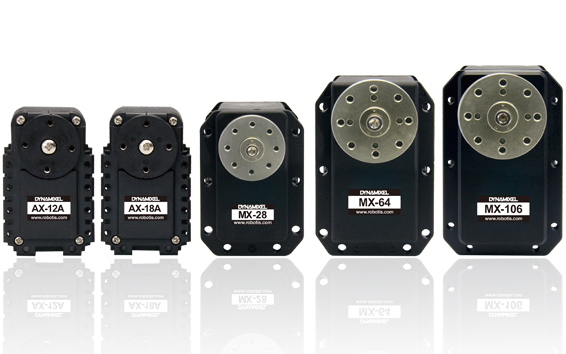
\includegraphics[width=0.48\linewidth]{dynamixel_actuator.jpg}}
    \hfil
    \subfloat[][Power of each Dynamixel model]{\label{fig:dynamixel_powa}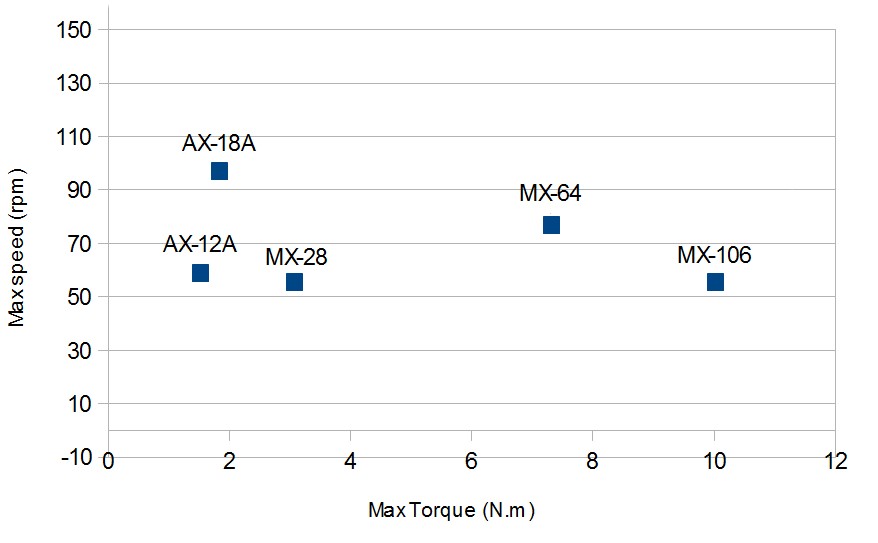
\includegraphics[width=0.48\linewidth]{comparaison-servomoteurs-dynamixel-robotis.png}}\\
    \caption{The Robotis Dynamixel come with different models from low cost ones such as AX-12/18 to the most powerful MX-series with maxon motor and magnetic encoder.}
    \label{fig:dynamixel_serie}
\end{figure}

Different models are available and permit the adjustment of the actuation to the power required by the joint (see \figurename~\ref{fig:dynamixel_powa}). They are different in size and power but their API remains the same and we can easily switch from one to another without changing the code or the electronic integration. Yet, even if the size changes, the foot-print keeps the same pattern (see \figurename~\ref{fig:dynamixel_dimension}) which make easy-to-configure parametric mechanical parts, it just takes a couple of minute to transform a part designed to be compatible with Dynamixel MX-28 to one compatible with Dynamixel MX-64.


\begin{figure}[tb]
    \begin{center}
        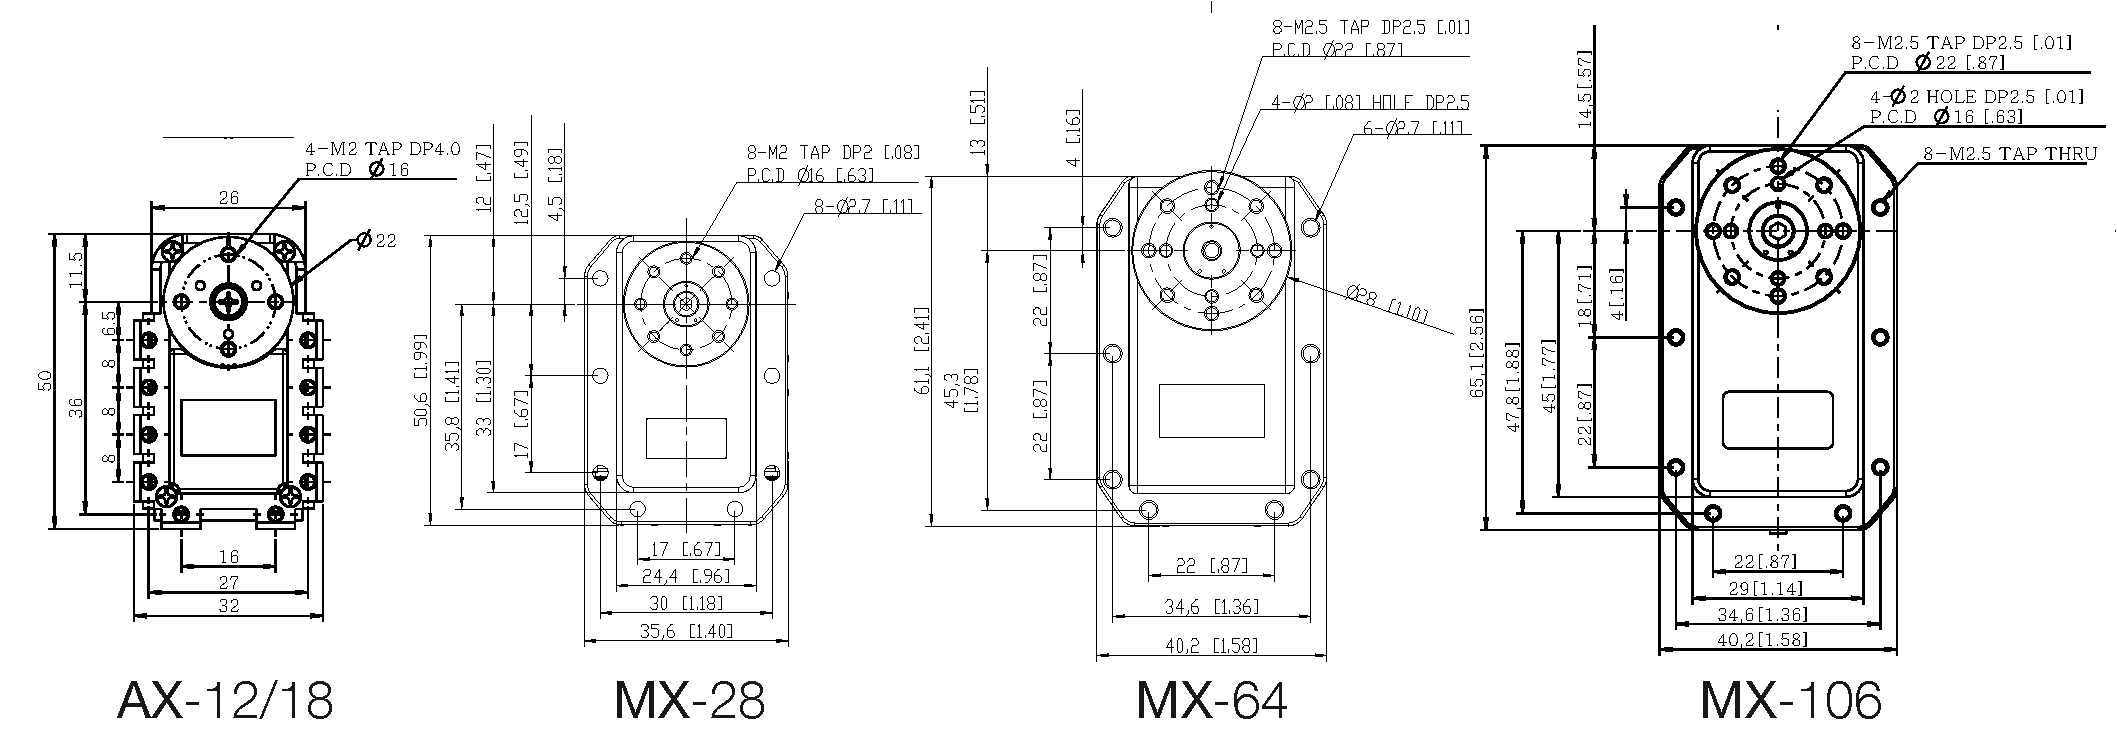
\includegraphics[width=\linewidth]{dynamixel_dimension.pdf}
    \end{center}
    \caption{The footprint of Dynamixel motors keeps the same pattern, only the dimensions are increased following the power of the motor. Thus, switching from one model to another only requires changing the dimension and not the design of a part. With parametric CAD software such as as Solidworks, it takes a couple of minutes to modify a mechanical part to be compatible with another Dynamixel motor.}
    \label{fig:dynamixel_dimension}
\end{figure}


\subsection{Accessible and extensible software} % (fold)

Having variables in software is more classical, yet using a non-stationary robot hardware (i.e. those link length or sensorimotor space can change) requires to have control library adapted to this low-level modularity. Here the choice has been made in favour of ease-of-use and modularity. We designed sensory-motor control API adapted to the hardware variability we have. We choose to use Python as the main programming language as it allows fast development, easy deployment on all operating systems and quick scripting by non-necessary expert developers. It also offers a large variety of scientific and machine-learning libraries used in robotics (e.g. Numpy, Scipy, Scikit-learn).
This language is rather slow compared to C or Java, but sensorimotor control is done using serial bus communication and as the serial communication is handled through the standard library we can still achieve rather high performance.

\subsection{Open source distribution} % (fold)

Finally, while the main aspect of such an approach is to allow variability, reuse and modification of the initial design, it is necessary to not only diffuse our work through scientific publications but also to distribute the material needed.
This means anyone outside the Flowers lab should have access to the actual source files and be free to make any changes suitable to their own research. Therefore in addition to the technological choices previously presented, we decided to distribute all our work (both software and hardware) under open source licenses.
This is an essential step toward building new research tools that facilitate both scientific validation and cumulative science in robotics. We will discuss this in detail in the next section.


\section{Allowing cumulative and Open science} % (fold)
\label{sec:allow-cumulative-science}
As we explained previously, new design approaches and methods should be used to create robots with morphology that can be explored by the user. In addition, by choosing the relevant technologies, we can permit both  the easy exploration of morphological variants, and the transfer and exchange between research laboratories.

To head in this direction, an unfettered access to knowledge and the components associated (articles, data, software, materials, methods) is needed. Also, it is preferable that work can be built upon without asking permission and where the methodology is increasingly based on open collaboration.

A very well adapted tool is the open-source license, which allows the source code, blueprint or design to be used, modified and/or shared under defined terms and conditions. The terms and conditions are defined by several different licenses and the author can choose among them the one that best suits the level of freedom  with which he wants to distribute his work. These licenses are famous and widespread in software development and have started to be used for hardware over the last few years (see chapter REF).

Nevertheless, in Science the preferred distribution channel is still primarily based on paper publishing and only a few researchers distribute their work under open source license. It is surprising as the use of open source collaboration seems very desirable for scientific research, especially in the robotic field:

\begin{description}
    \item[Scientific validation]: Similarly to publishing detailed mathematical proofs, sharing materials associated with a robotics experiment permits serious peer-reviewing, fundamental for the scientific validation of our field.
    Indeed, robotics experimentation involves a large amount of material (both software and hardware), reviewers should be able to evaluate if the material and experimental setup are coherent with the results submitted.

    \item[Open Science:] We often use only one part of the data collected in an experiment. The open distribution of all material allows the reuse of experiments by other researchers, who can use the same data to extract alternatives or extend the initial results.
    It also permits access to all details and especially to the constant parameter tuning, very sensible for a number of algorithms.

    \item[Cumulative Science] Most of the time, only a scientific paper is published. If this paper presents an algorithm or a mechanism, interested researchers have to reverse-engineer the entire development process. Either the researcher will have to waste time on doing this or he will not use this work at all.
    Finally, it permits mutual aid between researchers, which helps to debug or improve performance.

\end{description}


Yet placing all material we have on the web with an open source license is not enough to achieve the goals previously mentioned. As a paper has to be well written in a clear, precise and concise manner, associated material has to be understood and directly usable.
Therefore, there is a considerable amount of extra work required to permit fluent and effective open collaboration:
\begin{itemize}
    \item Since the work is intended to be reused by external and hopefully numerous of people, the sources have to be clean, robust and well-documented. In addition, some how-to tutorials are very welcome.
    \item A versioning tool should be set up to track changes and efficiently manage a collaborative workflow.
    \item Online community tools should be set up to host discussions between researchers.
\end{itemize}

This work can increase the overall development time by a factor of 3 but participates both in building cumulative science in the research community and increasing the actual impact of our work.

In the Poppy project we decided to distribute all the hardware under "copyleft" licenses, which let users freely use the sources as they want on the condition that they share the derivative work with the same license.
The open source distribution and community management will be discussed with more details in the chapter~\ref{cha:diffusion}.


\section{Conclusion} % (fold)

In this thesis, we aim to enable both the free exploration of morphological variants on real robotic platforms and their diffusion in the research community. To do so, we suggest exploring an alternative design based on 3D printing for mechanical parts, Arduino electronic architecture for sensors, Robotis Dynamixel motor for actuation and Python API for control.

This design process permits the creation of low-cost and highly hackable experimental robotic platforms thanks to a fully modular and open source approach.

The tools used form part of the makers revolution and the emergence of the new rapid prototyping tools, sometimes called the novel industrial revolution~\parencite{anderson2012makers}. Therefore we can rely on the hundreds of Fablabs around the world as a lever arm to increase the dissemination and reproducibility of robotic platforms designed with such methods.

Yet the chosen approach raised some limitations. Indeed, since we want to keep our work reproducible, we have to reduce the complexity of the assembly as well as the use of our robotic platforms. This means we need to spend more time developing and testing our design to make it as easy to use as possible. Also we are limited in the components we can use, they have to be easily accessible i.e. easily available and in large quantities in online stores.

Also, for the open source distribution, essential in creating a research community platform, a lot of effort is required to create an efficient and pleasant workflow.

In the next chapter, we will explain how we applied the methodology presented to the design of a whole new humanoid robot called Poppy. Then, the design of an easy-to-use modular Python library will be describe in chapter~\ref{cha:pypot}.





